\section{Video game development as software development} \label{game-development-sw}
\paragraph{Successful software}
Game development is a branch of software development, however, many argue that it is a separate genre
due to its completely different working pipelines and different composition of development teams, let alone the challenges 
related to project funding. A nicely written code, good functionality and user experience, fulfilling business specifications 
and remaininig within budget are usually enough for any commercial software to be successful on the market. In case of game 
development there are other factors that could potentially undermine the process leading to commercial failures.
\paragraph{Successful video game}
In fact, the end product of game development is mostly an entertainment or educational software. Apart from the code 
base that is basically the essence of any software product, the success of video games requires artistic assets, 
gameplay elements and also an immersive storyline or world creation fitting seamlessly together.
These components bring game development closer to creative industries like filmmaking. Actually, it is quite easy to mess
up any of the previously described elements or the interactions between them. 
A video game aiming to be a top-tier product cannot have good controls but horrible graphics
or beautiful graphics but nasty gameplay dynamics. Additionally, a good story helps to retain users so that
they do not turn away from the game too soon. On the other hand, there are many games considered as successful without
nice graphics or story, simply because they are "fun" to play. There is no formal way to define "fun", hence it becomes
a difficult task to define the ultimate definition of "good" or "succesful" video games, just like in case of movies.

\paragraph{Team composition}
The additional components to be considered in the game development workflow also affects team composition. The traditional
software development teams usually comprise the following roles: UI designer, UI developer, front-end and back-end developers,
product manager, database and system administrators, dev-ops, quality assurance (testers). Whereas in game development teams
other roles show up on top of the previous list, mostly related to artistic work: art teams designin 2D/3D objects 
(separate developers for game menus and other assets), animation teams, producer, game designer, content writer 
\cite{team-composition}.

\paragraph{Version control in game development}
The previously mentioned characteristics of video game production and team composition affect also the version controlling 
activities applied during development. Different teams have different needs and a good VCS can make their interactions smoother 
by adding as little additional administrative burden as possible while speeding up development cycles. The version control
system needs to be able to handle and integrate the work of art teams and game designers into traditional software development
workflow.
There are several options available when it comes to decide which version control system to use. The below chart shows 
the distribution of VCS among game developers.
\begin{figure}[H]
    \centering
    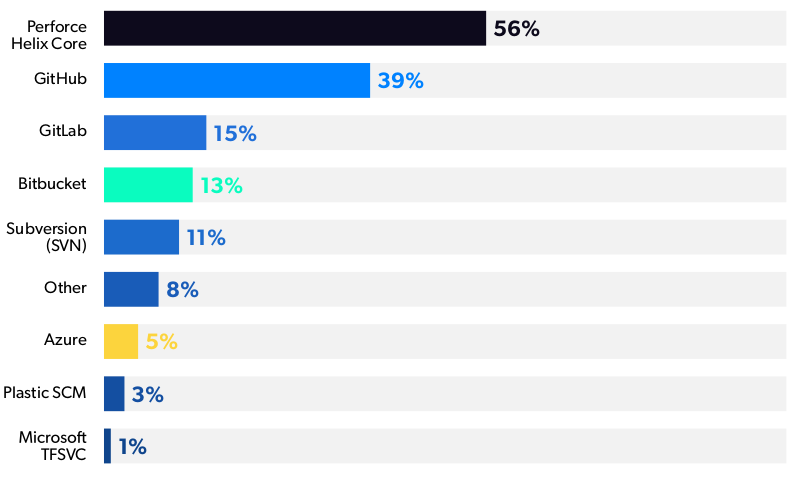
\includegraphics[width=\textwidth]{game-dev-survey-vcs.png}
    %\setlength{\belowcaptionskip}{-10pt}
    \caption{game dev survey vcs}
    \caption*{Source: The State of Game Development Report: 2020 $\&$ Beyond \protect\cite{game-dev-report-2020}}
    \label{fig:game-dev-survey-vcs}
\end{figure}

\paragraph{}
After the more theoretical first two sections of the paper, the next sections guide through a simple game development
project using the most widespread version control system of the industry, 
Helix Core\textsuperscript{\texttrademark}.